\documentclass[a4paper, 12pt]{article}
\usepackage{xeCJK}
    \setCJKmainfont[AutoFakeBold=1,AutoFakeSlant=.4]{標楷體}
    \XeTeXlinebreaklocale "zh"
    \XeTeXlinebreakskip = 0pt plus 1pt
\usepackage{fontspec}
    \setmainfont{Times New Roman}
\usepackage{setspace}
    \onehalfspace
    \setlength{\parskip}{1ex plus 0.5ex minus 0.2ex}
\usepackage{mathtools}
\usepackage{graphicx}
\usepackage{enumitem}
\usepackage{xcolor}
\parindent=0pt
\def\Large{\fontsize{16}{24}\selectfont}
\def\large{\fontsize{14}{20}\selectfont}
\makeatletter
\renewcommand\section{\@startsection {section}{1}{\z@}%
                                   {-3.5ex \@plus -1ex \@minus -.2ex}%
                                   {2.3ex \@plus.2ex}%
                                   {\centering\normalfont\Large\bfseries}}
\renewcommand\subsection{\@startsection {subsection}{1}{\z@}%
                                   {-3.5ex \@plus -1ex \@minus -.2ex}%
                                   {2.3ex \@plus.2ex}%
                                   {\centering\normalfont\large\bfseries}}
\makeatother
\begin{document}

\section*{資料來源}
\subsection*{空氣品質監測資料}
自2017年1月1日至2017年12月31日的高雄左營地區空氣品質觀測資料,取自於行政院環境保護署空氣品質監測網(https://taqm.epa.gov.tw/taqm/tw/YearlyDataDownload.aspx),當中包含每日每小時的各項監測濃度,我們取用其中的PM2.5、PM10、NO$_\textrm{2}$、NO、SO$_\textrm{2}$、CO與O$_\textrm{3}$,並計算每日的平均值作為當日監測資料。
\subsection*{蕁麻疹就診人數資料}
資料來自高雄榮民總醫院(皮膚科),為2017年1月1日至2017年12月31日診斷 ICD-9 代碼為708(蕁麻疹)每日就診人數資料,此篇為蕁麻疹的結果。

\section*{univariate gam}
Generalized additive Poisson model
$$
\ln (patient)=Intercept+\beta \times Airpollution+s(temperature)+s(humidity)+s(time)
$$
s= a cyclic cubic regression splines\\
下列依不同的空汙指標分別做單變數 Generalized additive Poisson model,並以時間趨勢、當天的溫度與濕度作為共變量做平滑函數的擬合,下列各空汙列出了不同的滯後天數(row,當天~前七天
)與不同的移動平均天數(colum,當天平均~七天平均)的模型結果(p-value與空汙估計係數)
\subsection*{CO}
下列以一氧化碳的分析結果來解釋。\\
Table1為空氣汙染的滯後效應與移動平均值來做gam 所得到的p-value\\
直行為不同的滯後效應的p-value結果\\
1-1的值(0.246)為當天的空汙數值與當天就診人數的gam p-value\\
2-1的值(0.683)為一天前的空汙數值與當天就診人數的gam p-value\\
3-1的值(0.002)為兩天前的空汙數值與當天就診人數的gam p-value\\
橫列為不同的天數做移動平均與當天的就診人數的gam p-value\\
1-1的值(0.246)今天的空汙數值與今天的就診人數所做的模型 p-value\\
1-2的值(0.728)今天+昨天的空汙平均值與今天的就診人數所做的模型 p-value\\
1-3的值(0.735今天+昨天+前天的空汙平均值與今天的就診人數所做的模型 p-value\\
目前我以p-value作為選擇標準,選取最小的p-value作為當前的解釋模型(紅色標記)
\begin{table}[h]
\centering
\caption{linear term p-value with lag and moving average data}
\begin{tabular}{rrrrrrrr}
  \hline
 & p.pv & mv2 & mv3 & mv4 & mv5 & mv6 & mv7 \\
  \hline
1 & 0.246 & 0.728 & 0.735 & 0.445 & 0.371 & 0.688 & 0.916 \\
  2 & 0.683 & 0.638 & 0.935 & 0.814 & 0.369 & 0.249 & 0.426 \\
  3 & \textcolor{red}{0.002} & 0.105 & 0.071 & 0.175 & 0.159 & 0.031 & 0.012 \\
  4 & 0.084 & 0.002 & 0.026 & 0.023 & 0.082 & 0.080 & 0.014 \\
  5 & 0.409 & 0.266 & 0.029 & 0.105 & 0.074 & 0.178 & 0.190 \\
  6 & 0.776 & 0.424 & 0.290 & 0.043 & 0.088 & 0.038 & 0.071 \\
  7 & 0.203 & 0.269 & 0.241 & 0.216 & 0.046 & 0.102 & 0.052 \\
  8 & 0.115 & 0.276 & 0.375 & 0.664 & 0.889 & 0.485 & 0.602 \\
   \hline
\end{tabular}
\\row:lag days,col:moving average for the n days
\end{table}
\begin{table}[h]
Table2為每個模型的空汙係數估計值,以我挑選的滯後兩天為例,0.977代表此空汙若上升一單位,就診人數便上升0.977單位\\
\centering
\caption{Parametric coefficients with lag and moving average data}
\begin{tabular}{rrrrrrrr}
  \hline
 & beta & mv2 & mv3 & mv4 & mv5 & mv6 & mv7 \\
  \hline
1 & 0.366 & 0.132 & 0.145 & 0.366 & 0.484 & 0.243 & -0.070 \\
  2 & -0.130 & 0.176 & 0.035 & 0.113 & 0.483 & 0.695 & 0.525 \\
  3 & \textcolor{red}{0.977} & 0.603 & 0.752 & 0.645 & 0.758 & 1.295 & 1.656 \\
  4 & 0.543 & 1.158 & 0.932 & 1.074 & 0.934 & 1.054 & 1.627 \\
  5 & 0.264 & 0.420 & 0.919 & 0.771 & 0.959 & 0.812 & 0.865 \\
  6 & 0.092 & 0.303 & 0.447 & 0.959 & 0.911 & 1.245 & 1.188 \\
  7 & 0.410 & 0.423 & 0.501 & 0.591 & 1.068 & 0.980 & 1.279 \\
  8 & -0.519 & -0.422 & -0.384 & -0.210 & -0.075 & 0.420 & 0.344 \\
   \hline
\end{tabular}
\end{table}

另外每個模型皆有加入溫度、濕度與時間趨勢的影響,在這裡將這些因素用平滑函數來估計對就診人數的影響力。以溫度來說,在不同的溫度對就診人數有不同的影響,例如:在太熱或太冷的時候對就診人數的影響較大,但在適合人類活動的溫度下影響較低。
\\
\clearpage
\begin{figure}
       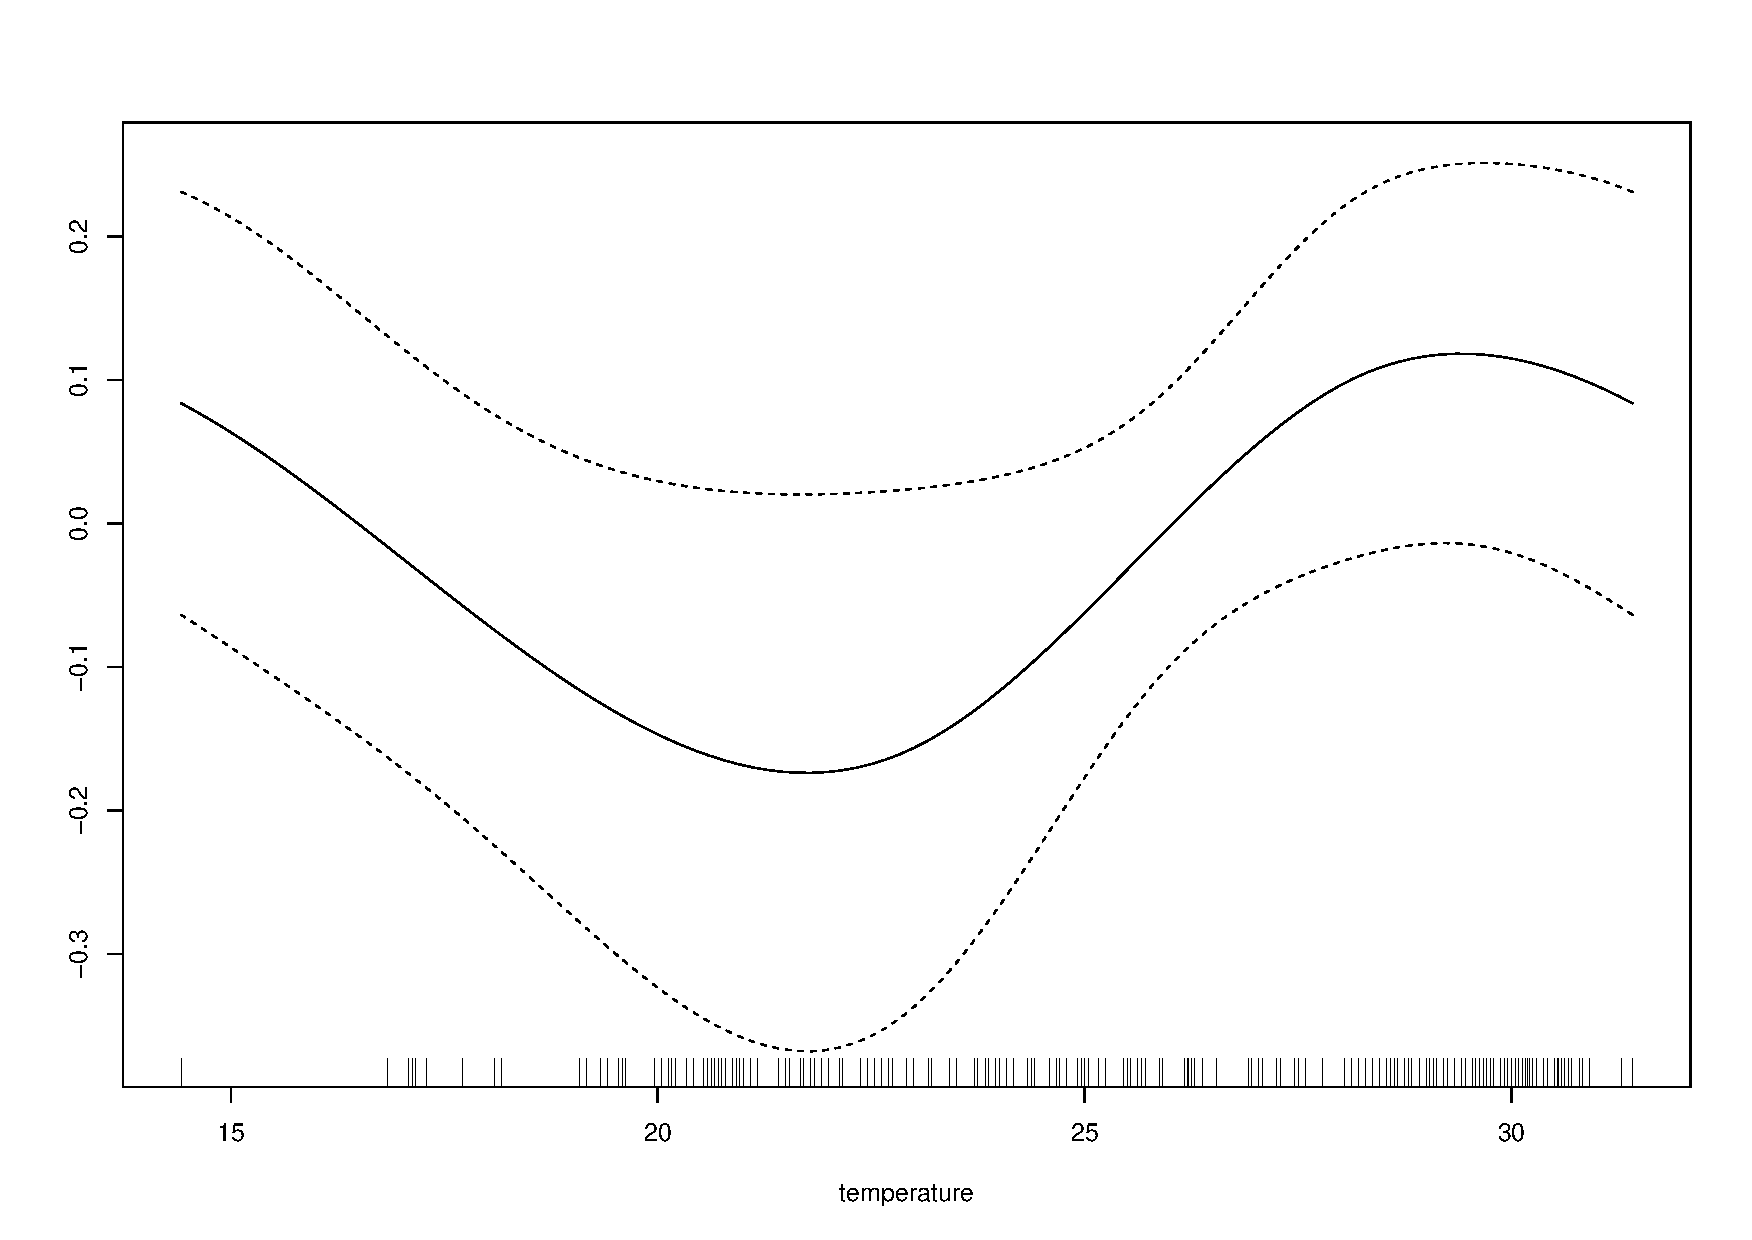
\includegraphics[width=13cm]{CO_temp.pdf}
       \caption{\label{}溫度對就診人數的影響,X軸為溫度,刻度為實際資料點(某天的溫度,共249天不包含假日),Y軸為對就診人數的影響,虛線為估計值的95\%信賴區間。以溫度來說,在大約20至23度時一氧化碳與就診人數為負相關,而在溫度28、29度時一氧化碳與就診人數有正向關係,也就是說在溫度越高時,一氧化碳的數值越高,就診人數也隨著變高。不過看到虛線部分,其信賴區間全包含$(y=0)$,這代表此因素並不顯著影響就診人數與一氧化碳的關係,意思是無論溫度多少,一氧化碳對就診人數的多寡是一樣的。在模型中溫度的平滑函數p-value為0.1764,也是未達顯著水準。}
\end{figure}
\begin{figure}
       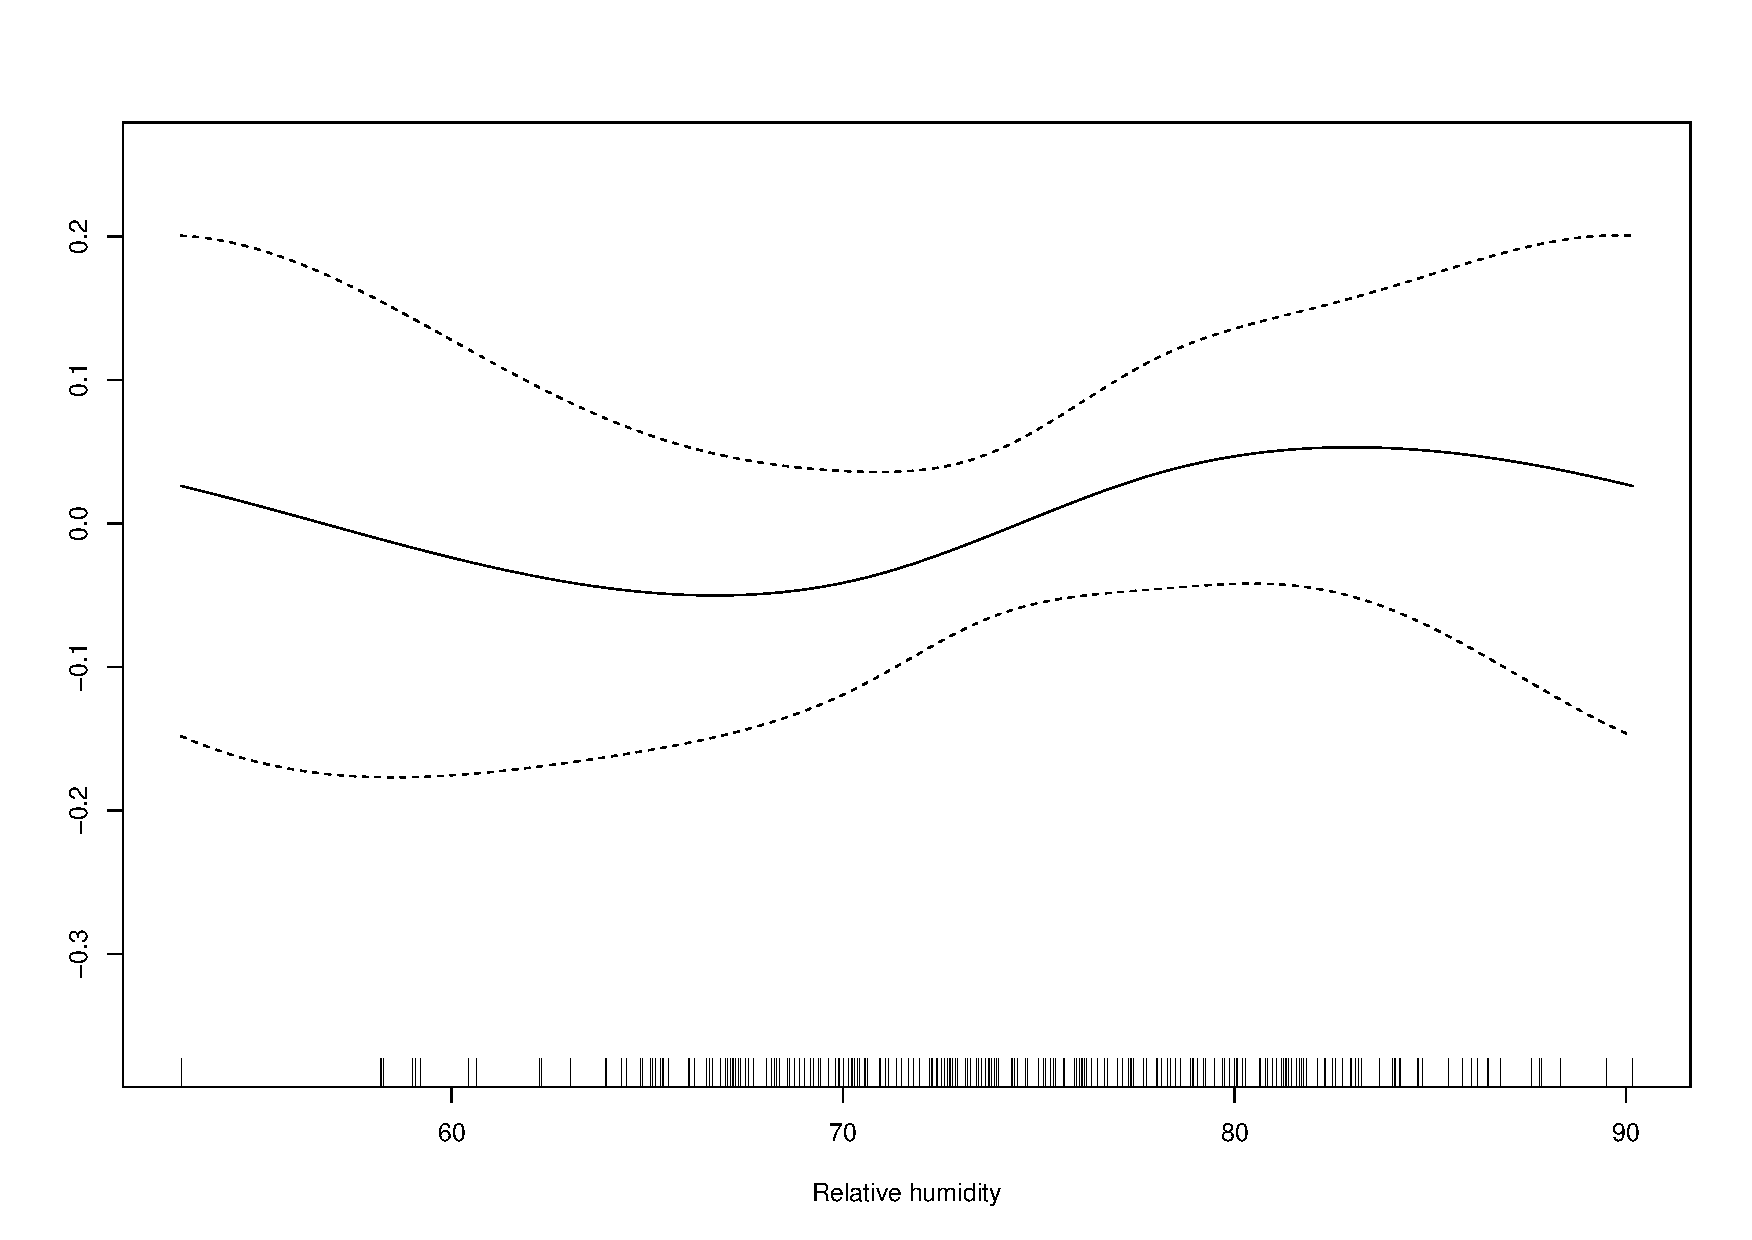
\includegraphics[width=13cm]{CO_RH.pdf}
       \caption{\label{}濕度對就診人數的影響,X軸為濕度,刻度一樣是實際資料點,整體看來比溫度的影響力更趨近水平線$(y=0)$。在模型中濕度的平滑函數p-value為0.5377,也是未達顯著水準。}
\end{figure}
\clearpage
\begin{figure}
       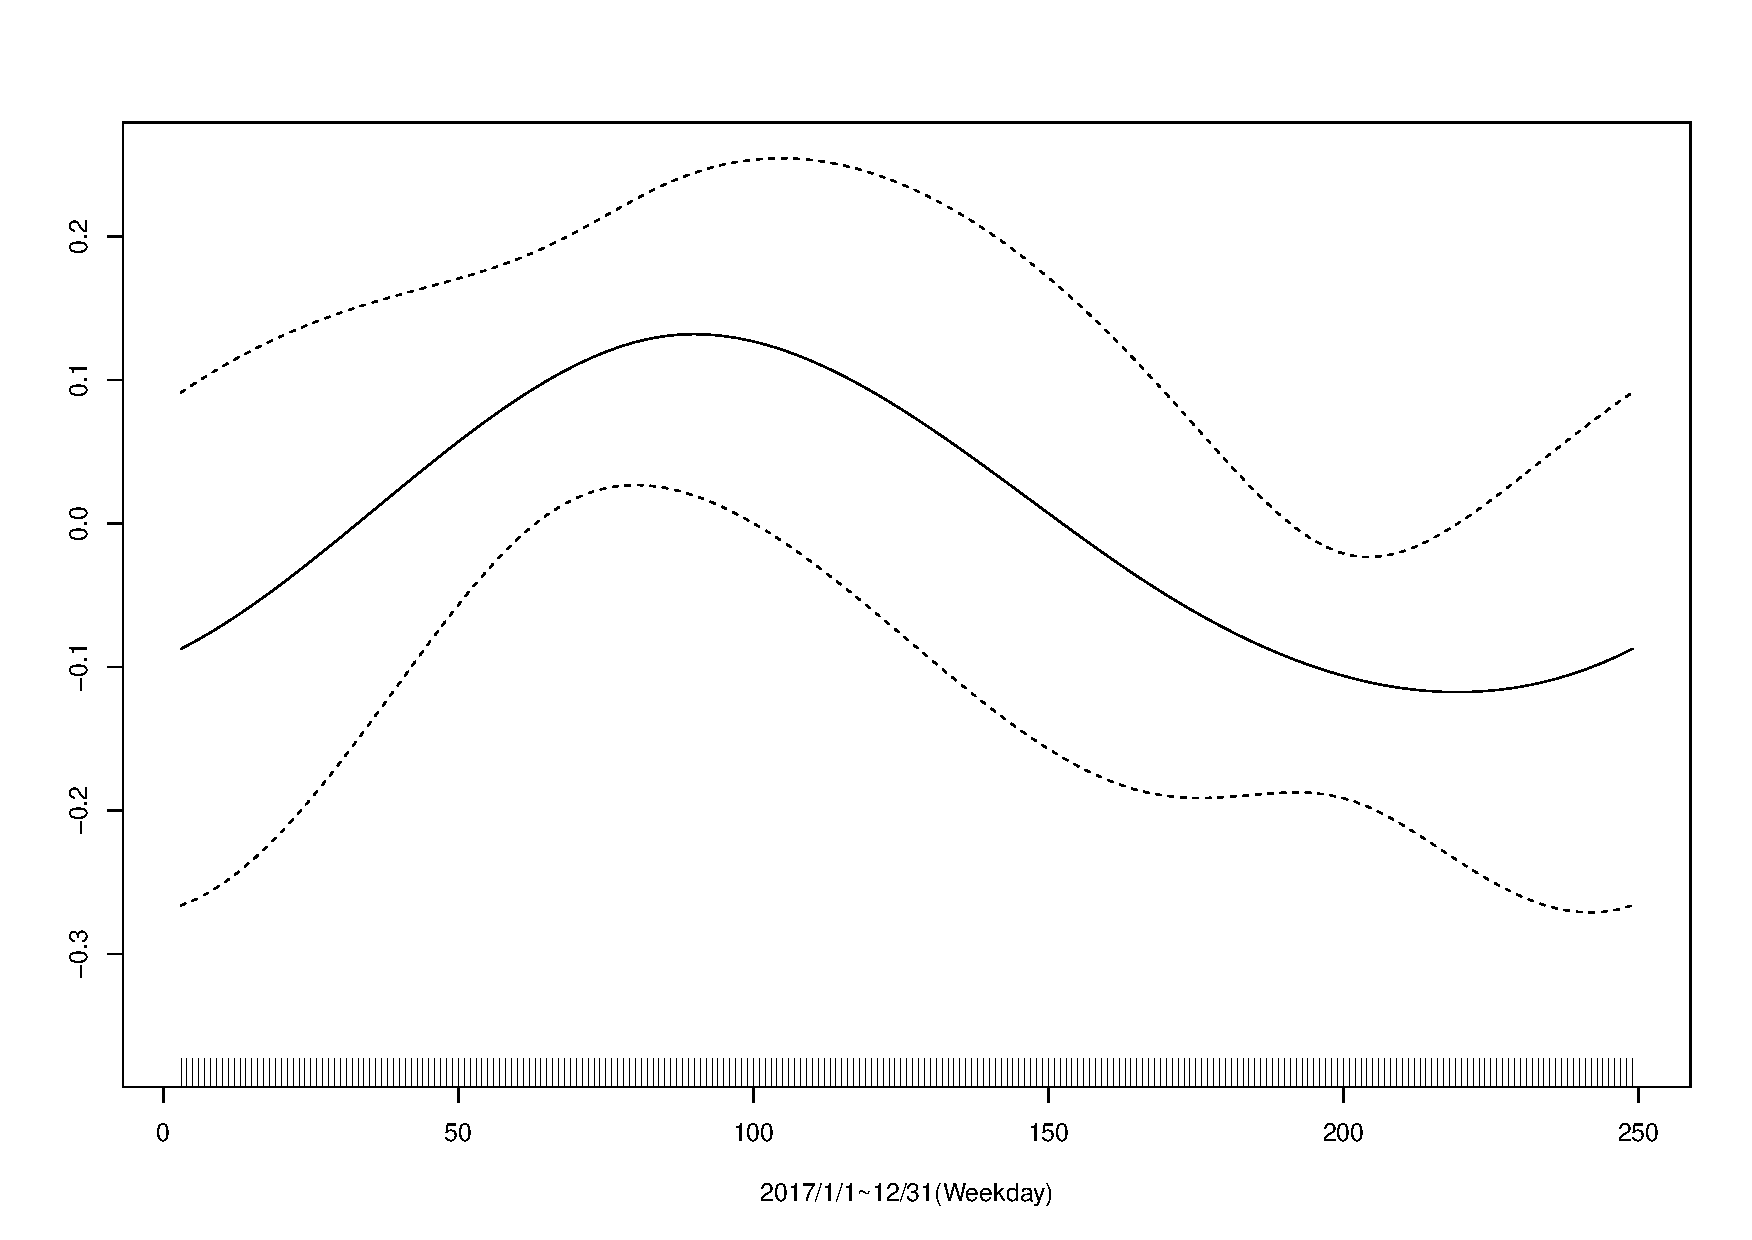
\includegraphics[width=13cm]{CO_time.pdf}
       \caption{\label{}時間對就診人數的影響,X軸為2017/1/1到2017/12/31日,刻度一樣是實際資料點,在X=(75,95)時(大約3、4月)一氧化碳對於就診人數的影響力是正相關,也就是一氧化碳數值越高,其就診人數有越高的趨勢,並且信賴區間也不包含$(y=0)$,一直到x=200附近(大約十月、十一月),一氧化碳的影響力變為負相關,亦即在這段時間一氧化碳濃度越高,其就診人數有相對較低的疑慮,發生這種問題可能是真正的影響因素為其他因素。在模型中溫度的平滑函數p-value為0.0307}
\end{figure}
\begin{figure}
下列兩張圖分別是每日就診人數與每日一氧化碳每日平均折線圖。
       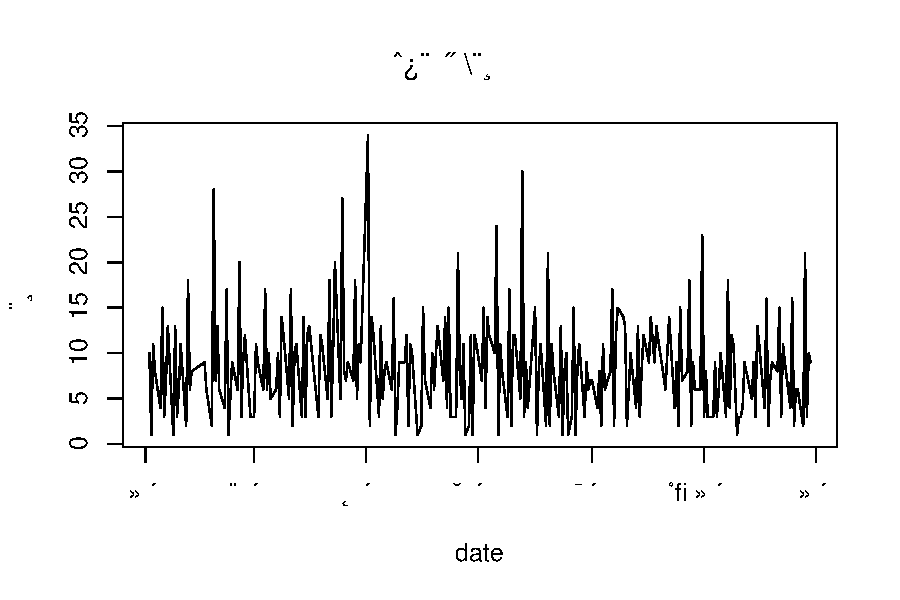
\includegraphics[width=13cm]{patient.pdf}
       \caption{\label{}每日就診人數}
       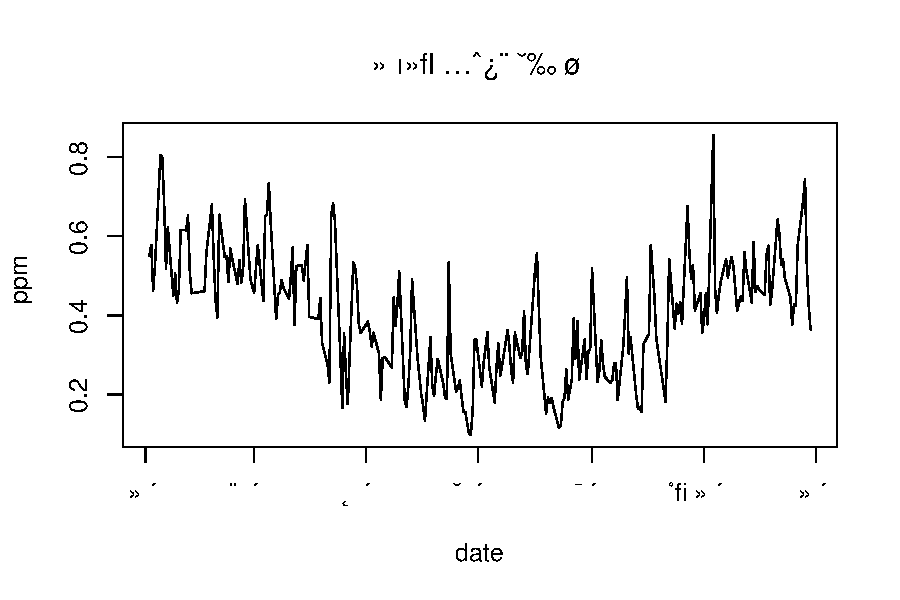
\includegraphics[width=13cm]{CO.pdf}
       \caption{\label{}每日一氧化碳平均值}
\end{figure}
\clearpage
\subsection*{SO2}
\begin{table}[h]
\centering
\caption{linear term p-value with lag and moving average data}
\begin{tabular}{rrrrrrrr}
  \hline
 & p.pv & mv2 & mv3 & mv4 & mv5 & mv6 & mv7 \\
  \hline
1 & 0.017 & 0.016 & 0.219 & 0.009 & 0.016 & 0.095 & 0.129 \\
  2 & 0.042 & 0.495 & 0.195 & 0.446 & 0.022 & 0.027 & 0.105 \\
  3 & \textcolor{red}{0.000} & 0.100 & 0.002 & 0.001 & 0.009 & 0.000 & 0.000 \\
  4 & 0.054 & 0.131 & 0.887 & 0.124 & 0.071 & 0.163 & 0.010 \\
  5 & 0.316 & 0.029 & 0.681 & 0.488 & 0.534 & 0.332 & 0.529 \\
  6 & 0.338 & 0.171 & 0.030 & 0.980 & 0.369 & 0.756 & 0.477 \\
  7 & 0.394 & 0.127 & 0.070 & 0.012 & 0.439 & 0.106 & 0.613 \\
  8 & 0.379 & 0.957 & 0.516 & 0.246 & 0.071 & 0.758 & 0.382 \\
   \hline
\end{tabular}
\\row:lag days,col:moving average for the n days
\end{table}

\begin{table}[h]
\centering
\caption{Parametric coefficients with lag and moving average data}
\begin{tabular}{rrrrrrrr}
  \hline
 & beta & mv2 & mv3 & mv4 & mv5 & mv6 & mv7 \\
  \hline
1 & 0.054 & 0.083 & 0.053 & 0.126 & 0.126 & 0.095 & 0.092 \\
  2 & -0.059 & 0.024 & 0.056 & 0.037 & 0.121 & 0.126 & 0.098 \\
  3 & \textcolor{red}{0.081} & 0.057 & 0.130 & 0.153 & 0.138 & 0.224 & 0.236 \\
  4 & -0.056 & 0.053 & 0.006 & 0.074 & 0.095 & 0.080 & 0.155 \\
  5 & -0.028 & -0.085 & 0.018 & -0.034 & 0.033 & 0.055 & 0.038 \\
  6 & -0.026 & -0.052 & -0.098 & -0.001 & -0.048 & 0.018 & 0.043 \\
  7 & -0.023 & -0.058 & -0.081 & -0.125 & -0.041 & -0.093 & -0.031 \\
  8 & 0.021 & -0.002 & -0.029 & -0.057 & -0.097 & -0.018 & -0.053 \\
   \hline
\end{tabular}
\end{table}
\clearpage
\subsection*{O3}
\begin{table}[h]
\centering
\caption{linear term p-value with lag and moving average data}
\begin{tabular}{rrrrrrrr}
  \hline
 & p.pv & mv2 & mv3 & mv4 & mv5 & mv6 & mv7 \\
  \hline
1 & 0.376 & 0.331 & 0.441 & 0.366 & 0.125 & 0.173 & 0.091 \\
  2 & 0.042 & 0.046 & 0.055 & 0.084 & 0.069 & 0.021 & 0.031 \\
  3 & 0.218 & 0.054 & 0.042 & 0.049 & 0.071 & 0.064 & 0.026 \\
  4 & \textcolor{red}{0.004} & 0.028 & 0.022 & 0.032 & 0.047 & 0.087 & 0.093 \\
  5 & 0.667 & 0.049 & 0.078 & 0.047 & 0.041 & 0.043 & 0.060 \\
  6 & 0.179 & 0.881 & 0.196 & 0.166 & 0.085 & 0.063 & 0.054 \\
  7 & 0.781 & 0.452 & 0.898 & 0.367 & 0.281 & 0.155 & 0.106 \\
  8 & 0.574 & 0.834 & 0.636 & 0.959 & 0.267 & 0.155 & 0.059 \\
   \hline
\end{tabular}
\\row:lag days,col:moving average for the n days
\end{table}

\begin{table}[h]
\centering
\caption{Parametric coefficients with lag and moving average data}
\begin{tabular}{rrrrrrrr}
  \hline
 & beta & mv2 & mv3 & mv4 & mv5 & mv6 & mv7 \\
  \hline
1 & 0.002 & 0.003 & 0.002 & 0.003 & 0.005 & 0.005 & 0.006 \\
  2 & 0.005 & 0.005 & 0.006 & 0.005 & 0.006 & 0.008 & 0.008 \\
  3 & 0.003 & 0.005 & 0.006 & 0.006 & 0.006 & 0.006 & 0.008 \\
  4 & \textcolor{red}{0.007} & 0.006 & 0.007 & 0.007 & 0.006 & 0.006 & 0.006 \\
  5 & 0.001 & 0.005 & 0.005 & 0.006 & 0.007 & 0.007 & 0.007 \\
  6 & -0.003 & -0.000 & 0.004 & 0.004 & 0.006 & 0.006 & 0.007 \\
  7 & -0.001 & -0.002 & -0.000 & 0.003 & 0.004 & 0.005 & 0.006 \\
  8 & -0.001 & -0.001 & -0.001 & 0.000 & 0.004 & 0.005 & 0.007 \\
   \hline
\end{tabular}
\end{table}
\clearpage
\subsection*{PM2.5}
\begin{table}[h]
\centering
\caption{linear term p-value with lag and moving average data}
\begin{tabular}{rrrrrrrr}
  \hline
 & p.pv & mv2 & mv3 & mv4 & mv5 & mv6 & mv7 \\
  \hline
1 & 0.004 & 0.316 & 0.729 & 0.212 & 0.464 & 0.656 & 0.852 \\
  2 & 0.960 & 0.114 & 0.663 & 0.972 & 0.282 & 0.501 & 0.606 \\
  3 & \textcolor{red}{0.000} & 0.003 & 0.000 & 0.013 & 0.050 & 0.005 & 0.019 \\
  4 & 0.041 & 0.000 & 0.000 & 0.000 & 0.003 & 0.016 & 0.001 \\
  5 & 0.518 & 0.129 & 0.001 & 0.004 & 0.001 & 0.012 & 0.045 \\
  6 & 0.543 & 0.837 & 0.263 & 0.004 & 0.008 & 0.001 & 0.007 \\
  7 & 0.970 & 0.846 & 0.763 & 0.314 & 0.012 & 0.015 & 0.001 \\
  8 & 0.799 & 0.812 & 0.581 & 0.845 & 0.568 & 0.034 & 0.029 \\
   \hline
\end{tabular}
\\row:lag days,col:moving average for the n days
\end{table}

\begin{table}[h]
\centering
\caption{Parametric coefficients with lag and moving average data}
\begin{tabular}{rrrrrrrr}
  \hline
 & beta & mv2 & mv3 & mv4 & mv5 & mv6 & mv7 \\
  \hline
1 & 0.009 & 0.004 & 0.002 & 0.007 & 0.004 & 0.003 & 0.001 \\
  2 & -0.000 & 0.006 & 0.002 & 0.000 & 0.006 & 0.004 & 0.004 \\
  3 & \textcolor{red}{0.015} & 0.012 & 0.017 & 0.013 & 0.011 & 0.018 & 0.016 \\
  4 & 0.006 & 0.018 & 0.017 & 0.022 & 0.018 & 0.015 & 0.022 \\
  5 & 0.002 & 0.006 & 0.016 & 0.015 & 0.020 & 0.016 & 0.014 \\
  6 & -0.002 & 0.001 & 0.005 & 0.015 & 0.016 & 0.022 & 0.019 \\
  7 & -0.000 & -0.001 & 0.001 & 0.005 & 0.015 & 0.016 & 0.023 \\
  8 & 0.001 & -0.001 & -0.003 & -0.001 & 0.003 & 0.014 & 0.015 \\
   \hline
\end{tabular}
\end{table}
\clearpage
\subsection*{PM10}
\begin{table}[h]
\centering
\caption{linear term p-value with lag and moving average data}
\begin{tabular}{rrrrrrrr}
  \hline
 & p.pv & mv2 & mv3 & mv4 & mv5 & mv6 & mv7 \\
  \hline
1 & 0.021 & 0.848 & 0.211 & 0.600 & 0.452 & 0.643 & 0.673 \\
  2 & 0.986 & 0.131 & 0.953 & 0.403 & 0.983 & 0.801 & 0.915 \\
  3 & \textcolor{red}{0.002} & 0.035 & 0.003 & 0.138 & 0.509 & 0.164 & 0.276 \\
  4 & 0.519 & 0.013 & 0.040 & 0.007 & 0.170 & 0.603 & 0.271 \\
  5 & 0.124 & 0.380 & 0.530 & 0.634 & 0.231 & 0.877 & 0.598 \\
  6 & 0.196 & 0.134 & 0.341 & 0.718 & 0.722 & 0.253 & 0.744 \\
  7 & 0.374 & 0.230 & 0.139 & 0.257 & 0.931 & 0.913 & 0.516 \\
  8 & 0.613 & 0.233 & 0.103 & 0.060 & 0.157 & 0.751 & 0.873 \\
   \hline
\end{tabular}
\\row:lag days,col:moving average for the n days
\end{table}

\begin{table}[h]
\centering
\caption{Parametric coefficients with lag and moving average data}
\begin{tabular}{rrrrrrrr}
  \hline
 & beta & mv2 & mv3 & mv4 & mv5 & mv6 & mv7 \\
  \hline
1 & 0.004 & -0.000 & -0.003 & -0.002 & -0.002 & -0.002 & -0.002 \\
  2 & -0.000 & 0.004 & -0.000 & -0.002 & -0.000 & -0.001 & 0.000 \\
  3 & \textcolor{red}{0.006} & 0.005 & 0.008 & 0.004 & 0.002 & 0.005 & 0.004 \\
  4 & 0.001 & 0.006 & 0.006 & 0.008 & 0.004 & 0.002 & 0.004 \\
  5 & -0.003 & -0.002 & 0.002 & 0.001 & 0.004 & 0.000 & -0.002 \\
  6 & -0.003 & -0.004 & -0.003 & 0.001 & 0.001 & 0.004 & 0.001 \\
  7 & -0.002 & -0.003 & -0.004 & -0.004 & -0.000 & -0.000 & 0.002 \\
  8 & -0.001 & -0.003 & -0.005 & -0.006 & -0.005 & -0.001 & -0.001 \\
   \hline
\end{tabular}
\end{table}
\clearpage
\subsection*{NO}
\begin{table}[h]
\centering
\caption{linear term p-value with lag and moving average data}
\begin{tabular}{rrrrrrrr}
  \hline
 & p.pv & mv2 & mv3 & mv4 & mv5 & mv6 & mv7 \\
  \hline
1 & 0.731 & 0.354 & 0.422 & 0.573 & 0.453 & 0.572 & 0.921 \\
  2 & \textcolor{red}{0.039} & 0.155 & 0.720 & 0.793 & 0.797 & 0.922 & 0.929 \\
  3 & 0.853 & 0.252 & 0.415 & 0.977 & 0.852 & 0.793 & 0.460 \\
  4 & 0.172 & 0.672 & 0.265 & 0.387 & 0.868 & 0.910 & 0.773 \\
  5 & 0.739 & 0.370 & 0.587 & 0.207 & 0.239 & 0.558 & 0.683 \\
  6 & 0.593 & 0.832 & 0.251 & 0.342 & 0.130 & 0.169 & 0.395 \\
  7 & 0.160 & 0.642 & 0.853 & 0.449 & 0.392 & 0.143 & 0.144 \\
  8 & 0.419 & 0.672 & 0.350 & 0.373 & 0.096 & 0.074 & 0.021 \\
   \hline
\end{tabular}
\\row:lag days,col:moving average for the n days
\end{table}

\begin{table}[h]
\centering
\caption{Parametric coefficients with lag and moving average data}
\begin{tabular}{rrrrrrrr}
  \hline
 & beta & mv2 & mv3 & mv4 & mv5 & mv6 & mv7 \\
  \hline
1 & -0.006 & 0.021 & 0.021 & 0.016 & 0.023 & 0.019 & 0.004 \\
  2 & \textcolor{red}{-0.041} & -0.034 & -0.009 & -0.008 & -0.008 & 0.003 & -0.003 \\
  3 & 0.003 & -0.027 & -0.022 & 0.001 & 0.006 & 0.009 & 0.026 \\
  4 & -0.027 & -0.010 & -0.030 & -0.026 & -0.005 & 0.004 & 0.010 \\
  5 & 0.006 & -0.021 & -0.014 & -0.037 & -0.038 & -0.020 & -0.015 \\
  6 & -0.010 & -0.005 & -0.031 & -0.028 & -0.049 & -0.047 & -0.031 \\
  7 & 0.025 & 0.011 & 0.005 & -0.022 & -0.027 & -0.050 & -0.053 \\
  8 & -0.015 & -0.010 & -0.025 & -0.026 & -0.053 & -0.060 & -0.083 \\
   \hline
\end{tabular}
\end{table}
\clearpage
\subsection*{NO2}
\begin{table}[h]
\centering
\caption{linear term p-value with lag and moving average data}
\begin{tabular}{rrrrrrrr}
  \hline
 & p.pv & mv2 & mv3 & mv4 & mv5 & mv6 & mv7 \\
  \hline
1 & 0.062 & 0.748 & 0.753 & 0.768 & 0.806 & 0.852 & 0.554 \\
  2 & 0.121 & 0.733 & 0.460 & 0.579 & 0.794 & 0.987 & 0.902 \\
  3 & \textcolor{red}{0.026} & 0.575 & 0.139 & 0.643 & 0.617 & 0.228 & 0.300 \\
  4 & 0.594 & 0.216 & 0.723 & 0.301 & 0.909 & 0.845 & 0.411 \\
  5 & 0.865 & 0.321 & 0.923 & 0.580 & 0.902 & 0.540 & 0.578 \\
  6 & 0.746 & 0.832 & 0.606 & 0.830 & 0.755 & 0.731 & 0.778 \\
  7 & 0.485 & 0.515 & 0.780 & 0.627 & 0.999 & 0.605 & 0.975 \\
  8 & 0.716 & 0.818 & 0.739 & 0.660 & 0.325 & 0.576 & 0.377 \\
   \hline
\end{tabular}
\\row:lag days,col:moving average for the n days
\end{table}

\begin{table}[h]
\centering
\caption{Parametric coefficients with lag and moving average data}
\begin{tabular}{rrrrrrrr}
  \hline
 & beta & mv2 & mv3 & mv4 & mv5 & mv6 & mv7 \\
  \hline
1 & 0.014 & -0.003 & -0.003 & 0.003 & -0.003 & -0.002 & -0.008 \\
  2 & -0.012 & 0.003 & -0.007 & -0.006 & 0.003 & -0.000 & 0.002 \\
  3 & \textcolor{red}{0.016} & 0.005 & 0.014 & 0.005 & 0.006 & 0.015 & 0.014 \\
  4 & -0.004 & 0.011 & 0.004 & 0.011 & 0.001 & 0.002 & 0.011 \\
  5 & -0.001 & -0.009 & 0.001 & -0.006 & 0.001 & -0.008 & -0.007 \\
  6 & 0.002 & 0.002 & -0.005 & 0.002 & -0.004 & 0.004 & -0.004 \\
  7 & 0.005 & 0.006 & 0.003 & -0.005 & -0.000 & -0.006 & 0.000 \\
  8 & 0.003 & -0.002 & -0.003 & -0.005 & -0.012 & -0.007 & -0.012 \\
   \hline
\end{tabular}
\end{table}
\clearpage



\end{document} 